\documentclass[10pt,a4paper,twocolumn]{article}

% ------------------------------------------------
% Packages
% ------------------------------------------------
\usepackage[utf8]{inputenc}
\usepackage[a4paper,margin=0.7in]{geometry}
\usepackage[runin]{abstract}
\usepackage{graphicx}
\usepackage{amsmath}
\usepackage{booktabs}
\usepackage{multirow}
\usepackage{tabularx}
\usepackage{array}
\usepackage{placeins}
\usepackage{caption}
\usepackage{setspace}
\usepackage{xcolor}
\usepackage{listings}

% ------------------------------------------------
% Formatting
% ------------------------------------------------
\setstretch{1.0}

\setlength{\textfloatsep}{8pt}
\setlength{\floatsep}{6pt}
\setlength{\intextsep}{6pt}

\captionsetup{
    font=small,
    labelfont=bf,
    skip=4pt
}

% ------------------------------------------------
% Code Styling
% ------------------------------------------------
\definecolor{codegreen}{rgb}{0,0.55,0}
\definecolor{codegray}{rgb}{0.45,0.45,0.45}
\definecolor{codepurple}{rgb}{0.58,0,0.82}
\definecolor{backcolour}{rgb}{0.97,0.97,0.97}

\lstset{
    backgroundcolor=\color{backcolour},
    commentstyle=\color{codegreen},
    keywordstyle=\color{blue},
    stringstyle=\color{codepurple},
    numberstyle=\tiny\color{codegray},
    basicstyle=\ttfamily\footnotesize,
    breaklines=true,
    breakatwhitespace=true,
    keepspaces=true,
    columns=flexible,
    frame=single,
    showstringspaces=false,
    xleftmargin=4pt,
    xrightmargin=4pt
}

% ------------------------------------------------
% Title
% ------------------------------------------------
\title{
\textbf{Design and Implementation of a 32-bit Single-Cycle RISC-V Processor}
}

\author{
\textbf{Hamza Arif} \\
Registration No: \textbf{2024206} \\
CE-222L --- Computer Organization and Assembly Language Lab
}

\date{\today}

% ------------------------------------------------
% Document
% --- Research paper style abstract ---
\renewcommand{\abstractnamefont}{\normalfont\bfseries\itshape}
\renewcommand{\abstracttextfont}{\normalfont\small}
\abslabeldelim{---}

\setlength{\absleftindent}{0pt}
\setlength{\absrightindent}{0pt}
% ------------------------------------------------
\begin{document}

\maketitle

% ------------------------------------------------
% Abstract
% ------------------------------------------------
\begin{abstract}
This report presents the design, implementation, and verification of a 32-bit single-cycle processor based on the RISC-V RV32I instruction set architecture using Verilog HDL. The processor supports arithmetic, logical, memory-access, and branch instructions within a unified single-cycle datapath. Major hardware modules including the Arithmetic Logic Unit (ALU), Register File, Control Unit, Immediate Generator, Instruction Memory, and Data Memory were implemented and tested individually before system integration. Simulation results demonstrate correct instruction execution and datapath behavior with a deterministic CPI of one. The project provides practical insight into processor datapath organization, instruction decoding, control signal generation, and hardware-level execution flow.
\end{abstract}

% ------------------------------------------------
\section{Introduction}

RISC-V is an open-standard instruction set architecture that has gained significant popularity in academia and industry because of its simplicity, modularity, and flexibility. Unlike proprietary architectures, RISC-V enables users to design custom processors without licensing restrictions, making it highly suitable for education and research.

The single-cycle processor is one of the most fundamental processor architectures used to understand CPU design principles. In this architecture, every instruction completes all five stages of execution --- Instruction Fetch (IF), Instruction Decode (ID), Execute (EX), Memory Access (MEM), and Write Back (WB) --- within a single clock cycle.

Although single-cycle processors are inefficient in terms of clock utilization, they provide a clean and simple implementation model that is ideal for understanding datapath routing, control signal generation, and instruction execution behavior.

The objective of this project is to design and implement a functional 32-bit RISC-V single-cycle processor capable of executing a subset of RV32I instructions using Verilog HDL and validating its operation through simulation.

% ------------------------------------------------
\section{Single-Cycle Architecture}

In a single-cycle processor, each instruction completes execution in exactly one clock cycle. Therefore, the clock period must be long enough to accommodate the slowest instruction path, which is usually a memory-access instruction such as \texttt{lw}.

The processor datapath integrates instruction fetch, decoding, execution, memory access, and write-back hardware into a single unified structure.

% ------------------------------------------------
\subsection{Advantages}

\begin{itemize}
    \item \textbf{Simple Datapath:} No pipeline registers, forwarding logic, or hazard detection mechanisms are required.
    
    \item \textbf{Deterministic CPI:} Every instruction executes in one cycle, resulting in a CPI of exactly 1.
    
    \item \textbf{Ease of Debugging:} Since the processor state updates only once per cycle, simulation and verification become simpler.
\end{itemize}

% ------------------------------------------------
\subsection{Limitations}

\begin{itemize}
    \item \textbf{Long Clock Period:} The clock frequency is limited by the slowest instruction execution path.
    
    \item \textbf{Inefficient Resource Usage:} Faster instructions waste unused cycle time while waiting for the clock edge.
    
    \item \textbf{Separate Memories Required:} Instruction and Data memory must be separated to allow simultaneous access.
\end{itemize}

% ------------------------------------------------
\section{Supported Instruction Set}

The implemented processor supports the following subset of RV32I instructions:

\begin{center}
\texttt{add, sub, and, or, lw, sw, beq}
\end{center}

These instructions cover:

\begin{itemize}
    \item Arithmetic operations
    \item Logical operations
    \item Memory access
    \item Conditional branching
\end{itemize}

% ------------------------------------------------
\subsection{Instruction Formats}

RISC-V instructions are fixed-width 32-bit instructions. The implementation supports four instruction formats.

\begin{table*}[t]
\centering
\caption{RISC-V Instruction Formats}
\label{tab:formats}

\begin{tabular}{|c|c|c|c|c|c|c|}
\hline
\textbf{Format} & \textbf{31:25} & \textbf{24:20} & \textbf{19:15} & \textbf{14:12} & \textbf{11:7} & \textbf{6:0} \\
\hline
R-type & funct7 & rs2 & rs1 & funct3 & rd & opcode \\
\hline
I-type & \multicolumn{2}{c|}{imm[11:0]} & rs1 & funct3 & rd & opcode \\
\hline
S-type & imm[11:5] & rs2 & rs1 & funct3 & imm[4:0] & opcode \\
\hline
B-type & imm[12,10:5] & rs2 & rs1 & funct3 & imm[4:1,11] & opcode \\
\hline
\end{tabular}
\end{table*}

% ------------------------------------------------
\subsection{Supported Encodings}

\begin{table*}[t]
\centering
\caption{Instruction Encodings}
\label{tab:encodings}

\begin{tabular}{|l|c|c|c|c|}
\hline
\textbf{Instruction} & \textbf{Type} & \textbf{Opcode} & \textbf{funct3} & \textbf{funct7} \\
\hline
\texttt{add} & R & 0110011 & 000 & 0000000 \\
\hline
\texttt{sub} & R & 0110011 & 000 & 0100000 \\
\hline
\texttt{and} & R & 0110011 & 111 & 0000000 \\
\hline
\texttt{or} & R & 0110011 & 110 & 0000000 \\
\hline
\texttt{lw} & I & 0000011 & 010 & N/A \\
\hline
\texttt{sw} & S & 0100011 & 010 & N/A \\
\hline
\texttt{beq} & B & 1100011 & 000 & N/A \\
\hline
\end{tabular}
\end{table*}

% ------------------------------------------------
\section{Processor Datapath}

The processor consists of multiple interconnected hardware modules responsible for different execution stages.

% ------------------------------------------------
\subsection{Program Counter and Instruction Fetch}

The Program Counter (PC) stores the address of the current instruction. During every cycle:

\begin{itemize}
    \item The instruction memory outputs the instruction stored at the current PC address.
    \item An adder increments the PC by 4 to point to the next instruction.
\end{itemize}

% ------------------------------------------------
\subsection{Register File}

The register file contains 32 general-purpose 32-bit registers.

\begin{itemize}
    \item Two registers can be read simultaneously.
    \item One register can be written during the write-back stage.
    \item Register \texttt{x0} is permanently hardwired to zero.
\end{itemize}

% ------------------------------------------------
\subsection{Immediate Generator}

The Immediate Generator extracts and sign-extends immediate values from I-type, S-type, and B-type instructions. Different instruction formats place immediate fields in different bit locations, requiring custom extraction logic.

% ------------------------------------------------
\subsection{Arithmetic Logic Unit (ALU)}

The ALU performs arithmetic and logical operations including:

\begin{itemize}
    \item Addition
    \item Subtraction
    \item Bitwise AND
    \item Bitwise OR
\end{itemize}

The ALU also generates a \texttt{Zero} signal used for branch decisions.

% ------------------------------------------------
\subsection{Data Memory}

The Data Memory module handles:

\begin{itemize}
    \item Load operations (\texttt{lw})
    \item Store operations (\texttt{sw})
\end{itemize}

The ALU output acts as the effective memory address.

% ------------------------------------------------
\begin{figure}[!t]
\centering
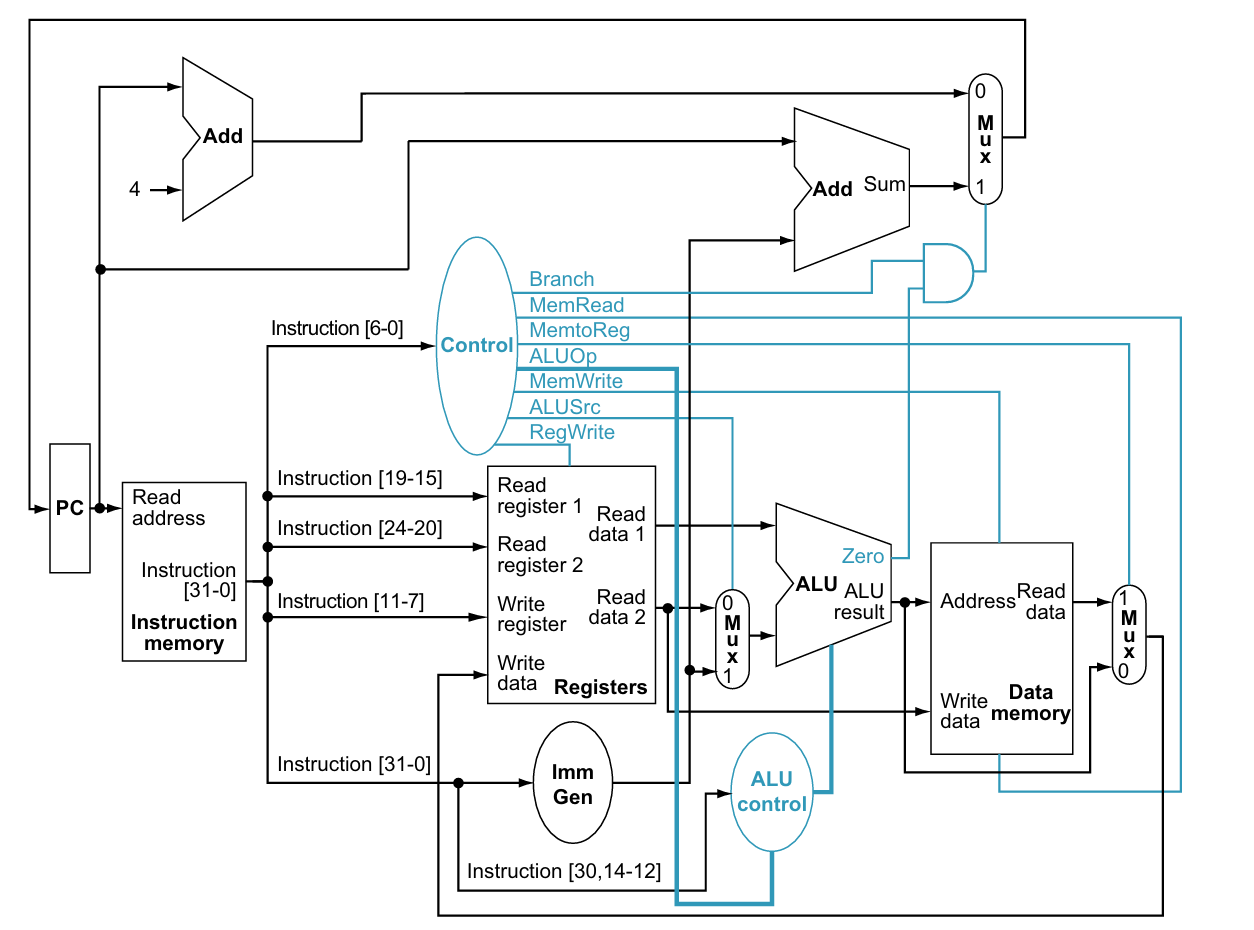
\includegraphics[width=\linewidth]{architecture.png}
\caption{Single-cycle RISC-V processor datapath.}
\label{fig:architecture}
\end{figure}

% ------------------------------------------------
\section{Control Unit}

The Main Control Unit generates datapath control signals based on the opcode field of the instruction.

\begin{table}[h]
\centering
\caption{Main Control Signals}

\resizebox{\columnwidth}{!}{
\begin{tabular}{|c|c|c|c|c|c|c|}
\hline
Instr & ALUSrc & MemtoReg & RegWrite & MemRead & MemWrite & Branch \\
\hline
R-type & 0 & 0 & 1 & 0 & 0 & 0 \\
\hline
lw & 1 & 1 & 1 & 1 & 0 & 0 \\
\hline
sw & 1 & X & 0 & 0 & 1 & 0 \\
\hline
beq & 0 & X & 0 & 0 & 0 & 1 \\
\hline
\end{tabular}
}
\end{table}

% ------------------------------------------------
\subsection{ALU Control Unit}

The ALU Control Unit combines:

\begin{itemize}
    \item ALUOp from the main controller
    \item funct3 field
    \item funct7 field
\end{itemize}

to determine the required ALU operation.

% ------------------------------------------------
\section{Instruction Execution Examples}

% ------------------------------------------------
\subsection{R-type Instruction Execution}

For the \texttt{add} instruction:

\begin{enumerate}
    \item Instruction is fetched from memory.
    \item Source registers are read.
    \item ALU performs addition.
    \item Result is written back to destination register.
\end{enumerate}

% ------------------------------------------------
\subsection{Load Instruction Execution}

For the \texttt{lw} instruction:

\begin{enumerate}
    \item Base register and immediate are decoded.
    \item ALU computes effective address.
    \item Data memory is accessed.
    \item Loaded data is written back to the register file.
\end{enumerate}

% ------------------------------------------------
\subsection{Branch Instruction Execution}

For the \texttt{beq} instruction:

\begin{enumerate}
    \item Source registers are compared using subtraction.
    \item If Zero = 1, branch target address is selected.
    \item Otherwise, execution continues sequentially.
\end{enumerate}

% ------------------------------------------------
\section{Verification and Testing}

The processor was verified using a custom Verilog testbench executed in Icarus Verilog. The following assembly test program was loaded into instruction memory.

\begin{center}
\begin{minipage}{0.95\columnwidth}

\begin{lstlisting}[language=Verilog,caption={Assembly Test Program}]
lw  x1, 0(x0)
lw  x2, 4(x0)

add x3, x1, x2
sub x4, x2, x1

sw  x3, 8(x0)

and x5, x3, x4
or  x6, x3, x4

beq x4, x1, 8

sw  x1, 12(x0)
sw  x2, 16(x0)
\end{lstlisting}

\end{minipage}
\end{center}

The test program validates arithmetic operations, logical operations, memory access, and conditional branching behavior.

% ------------------------------------------------
\section{Simulation Results}

Simulation outputs confirmed correct processor functionality.

\begin{figure}[!t]
\centering
\includegraphics[width=\linewidth]{terminal1.png}
\caption{Instruction execution trace.}
\label{fig:trace}
\end{figure}

\begin{figure}[!t]
\centering
\includegraphics[width=\linewidth]{terminal2.png}
\caption{Register file contents after execution.}
\label{fig:registers}
\end{figure}

\begin{figure}[!t]
\centering
\includegraphics[width=\linewidth]{terminal3.png}
\caption{Data memory contents after store operations.}
\label{fig:memory}
\end{figure}

\FloatBarrier

% ------------------------------------------------
\section{Waveform Analysis}

GTKWave timing analysis verified proper synchronization between the clock, program counter, instruction memory, ALU outputs, and register write-back signals.

The waveform confirmed:

\begin{itemize}
    \item Correct instruction sequencing
    \item Proper immediate generation
    \item Stable ALU outputs before clock transitions
    \item Correct branch resolution behavior
\end{itemize}

\begin{figure}[!t]
\centering
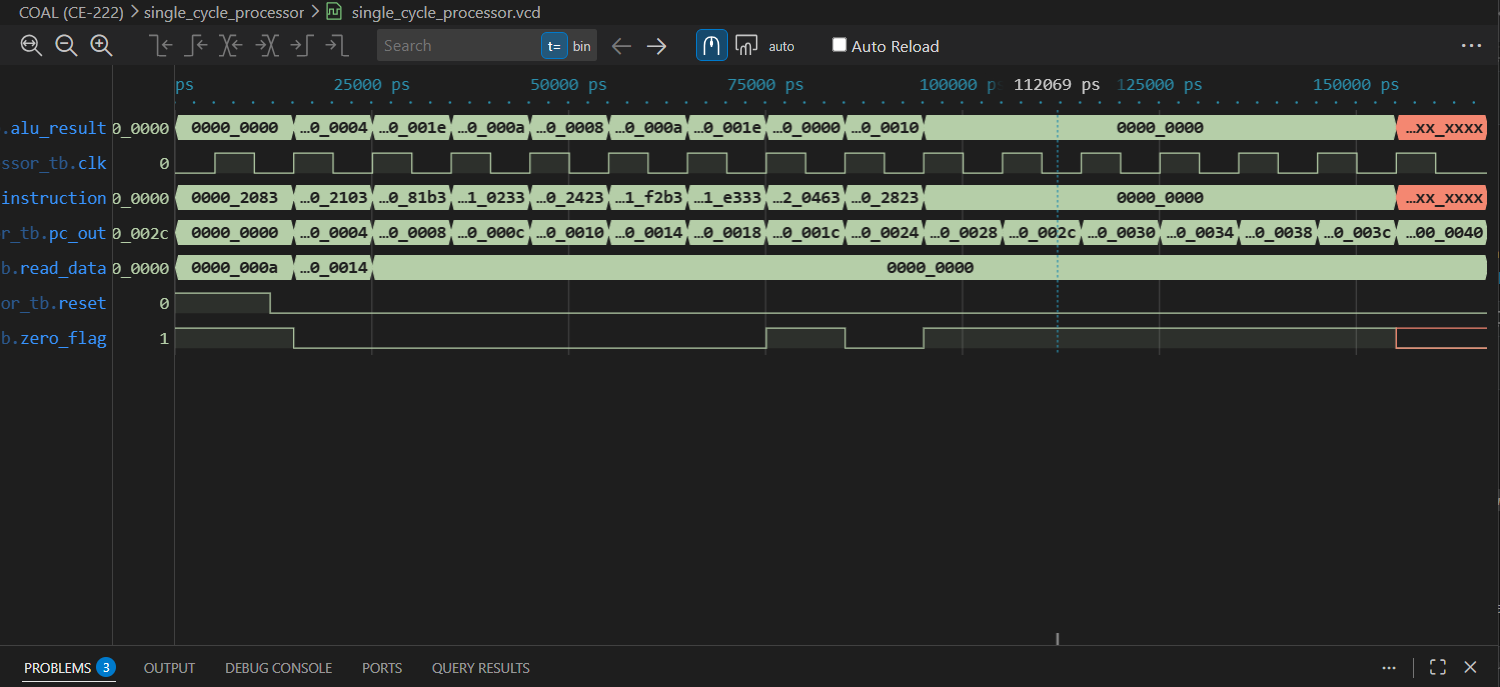
\includegraphics[width=\linewidth]{waveform.png}
\caption{Processor timing waveform in GTKWave.}
\label{fig:waveform}
\end{figure}

% ------------------------------------------------
\section{Conclusion and Future Work}

This project successfully implemented a functional 32-bit single-cycle RISC-V processor using Verilog HDL. The processor correctly executed arithmetic, logical, memory-access, and branch instructions from the RV32I instruction subset.

The implementation demonstrated fundamental concepts of processor design including datapath organization, control signal generation, instruction decoding, ALU operation, and memory interfacing.

Although the single-cycle architecture is simple and easy to understand, its long critical path limits performance. Future work will focus on converting the processor into a pipelined architecture with hazard detection and forwarding mechanisms to improve throughput and clock frequency.

% ------------------------------------------------
\end{document}